\begin{figure*}[t]
  \centering
  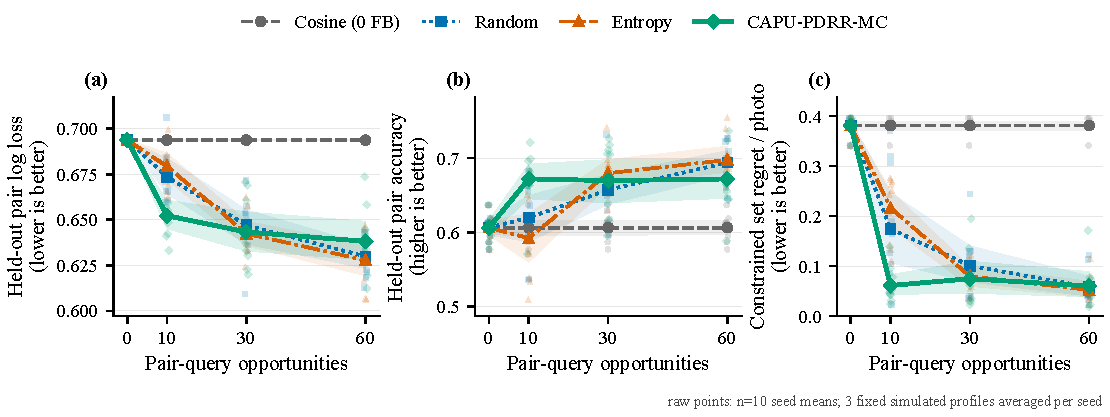
\includegraphics[width=0.95\textwidth]{figures/fig4_pdrr_acquisition_learning.pdf}
  \caption{Query-efficiency comparison for the 67D contextual preference adapter on 70 public Wikimedia images. Each replicate uses the source-pinned 42/28 exact-file-disjoint split; acquisition sees only the 42 training images. Lines are means across 10 split/choice seeds after averaging three fixed simulated profiles, shading gives 95\% percentile-bootstrap intervals, and faint points are raw seed means. CAPU-PDRR-MC uses $B=64$ posterior draws, a 16-pair shortlist, and an exact partition-constrained action re-solve. At budget 10, all paired PDRR-versus-random and PDRR-versus-entropy intervals favor PDRR; at budgets 30 and 60 all corresponding intervals cross zero. The evidence therefore supports low-budget sample efficiency, not universal or asymptotic superiority. Preferences are simulated rather than human-provided.}
  \label{fig:controlled-pdrr-acquisition}
\end{figure*}
